%=======================================================================
%  When Does Joint Admission Control and Routing Pay?
%  A Routing-Headroom Law for DRL-Based Core Network Slicing
%
%  DRAFT v3 -- restructured around the completed experiments (Oct 2026).
%
%  HOW TO USE THIS FILE
%  --------------------
%  Each paragraph slot has:
%     1. a "% [Px] GUIDANCE:" comment -- what the paragraph must argue,
%        which numbers to quote, what to cite;
%     2. a draft paragraph in plain prose.
%  Rewrite the prose in your own voice. Do not touch the LaTeX.
%  All tables/equations/algorithms are coded; all figures are external
%  PDFs in figures/ (regenerate with: python3 make_figures.py).
%
%  WHAT CHANGED FROM v2
%  --------------------
%  The rho sweep completed and the routing-headroom law now holds with
%  r^2 = 0.979 over five controlled levels. rho is therefore promoted
%  from a boundary condition to the paper's CENTRAL claim: title,
%  abstract, contributions and Section VI-C are built around it.
%  Added: the aggregate-state baseline (published-literature stand-in),
%  the factored-architecture result at rho=0, and the deployment rule.
%
%  !! See CLAIMS AUDIT at the end before submitting.
%=======================================================================
\documentclass[10pt,journal,comsoc]{IEEEtran}
\usepackage{amsmath,amsfonts}
\usepackage{algorithm}
\usepackage{array}
\usepackage{amssymb}
\usepackage{amsthm}
\usepackage[caption=false,font=normalsize,labelfont=sf,textfont=sf]{subfig}
\usepackage{textcomp}
\usepackage{stfloats}
\usepackage{url}
\usepackage{cite}
\usepackage{color}
\usepackage{multirow}
\usepackage{graphicx}
\usepackage{booktabs}
\usepackage{mathtools}
\newtheorem{definition}{Definition}
\usepackage{makecell}
\usepackage{algpseudocode}
\graphicspath{{figures/}}
\hyphenation{op-tical net-works semi-conduc-tor IEEE-Xplore}

\begin{document}

\title{When Does Joint Admission Control and Routing Pay?\\
A Routing-Headroom Law for Deep Reinforcement Learning\\
in Core Network Slicing}

\author{Pedro Amaral,~\IEEEmembership{Member,~IEEE}
\thanks{Pedro Amaral is with the Departamento de Engenharia Electrot\'ecnica e de Computadores, Faculdade de Ci\^encias e Tecnologia,
FCT/UNL, Universidade Nova de Lisboa, 2829-516 Caparica, Portugal; pfa@fct.unl.pt, and Instituto de Telecomunica\c{c}\~oes, 1049-001 Lisbon, Portugal}%
}

\markboth{IEEE Transactions on Network and Service Management,~Vol.~XX, No.~X, 2026}%
{Amaral: When Does Joint Admission Control and Routing Pay?}

\IEEEpubid{0000--0000/00\$00.00~\copyright~2026 IEEE}
\maketitle

%=======================================================================
\begin{abstract}
%-----------------------------------------------------------------------
% GUIDANCE (ABSTRACT). Argument order, with the measured numbers:
%  1. Context: AC and RA are coupled in the IP/MPLS transport core.
%  2. What we build: one DRL agent deciding admit/reject AND which of K
%     paths, state restricted to OSS/telemetry counters.
%  3. THE HEADLINE: whether learning to route pays is governed by a
%     substrate statistic rho, computable WITHOUT training. On a family
%     where rho is the only manipulated variable the joint-vs-AC-only
%     advantage is linear in rho: gap = 0.97*rho - 1.82, r^2 = 0.979,
%     from -1.7% at rho=0 to +12.7% at rho=14.4%.
%  4. Mechanism of the admission half: admissibility preservation --
%     54.9% vs 46.2% feasible arrivals (+8.7pp).
%  5. Against a published-literature-style aggregate-state controller we
%     gain +14.6%; of that, +6.7pp is the path-level state alone.
%  6. Architecture: the factored agent is never significantly worse than
%     admission-only (rho=0: -0.8%, n.s.) and significantly better where
%     routing matters (+5.9%), so it is the deployable choice.
%  DO NOT reinstate the old "47.5% more slices" / "18% more fulfilled".
%-----------------------------------------------------------------------
Network slicing requires an operator to decide, for each arriving slice
request, whether to admit it and how to embed it. In the IP/MPLS
transport core the two decisions are coupled, and it is widely assumed
that learning them jointly is preferable to learning admission alone. We
show that this is true only under a condition that can be measured in
advance. We formulate joint admission control and path-level resource
allocation as a Markov Decision Process whose state uses only counters
already exported by production OSS and telemetry systems, and solve it
with duelling deep Q-networks in a unified and a factored variant. We
then define the \emph{routing headroom} $\rho$ of a substrate -- the
fraction of arrivals admissible on some candidate path but not on the
shortest one -- and show, on a family of topologies in which $\rho$ is
the only manipulated variable and the operating point is held fixed,
that the advantage of joint control over admission-only control is
linear in $\rho$: it rises from $-1.7\%$ at $\rho=0$ to $+12.7\%$ at
$\rho=14.4\%$, with $r^2=0.979$. Two real substrates fall on the same
line. $\rho$ requires no training to evaluate, so an operator can decide
the architecture before committing to it. We further identify the
mechanism behind the admission half of the problem: the learned policy
preserves future admissibility, sustaining $54.9\%$ routable arrivals
against $46.2\%$ under a strong bottleneck-aware greedy policy. Against a
controller built on the aggregate resource state used in the 5G-core
literature, the joint agent admits $14.6\%$ more slices, of which
$6.7$ percentage points are attributable to the path-level state
representation alone. Finally, the factored architecture is never
significantly worse than an admission-only controller, including where
routing is provably useless, and significantly better where routing
matters, making it the architecture we recommend.
\end{abstract}
\IEEEpubidadjcol
\begin{IEEEkeywords}
Deep reinforcement learning, network slicing, admission control,
resource allocation, IP core networks, routing, generalization.
\end{IEEEkeywords}

%=======================================================================
\section{Introduction}
%=======================================================================
%-----------------------------------------------------------------------
% [I-P1] GUIDANCE: Motivation -- 5G/6G verticals over one substrate;
% slice management is the operator's control problem. Cite
% guan2021customized, bernardez2021machine. Keep it to 3-4 sentences.
%-----------------------------------------------------------------------
Next-generation networks must support services whose traffic profiles and
quality-of-service requirements differ by orders of magnitude. In the 5G
and beyond service model distinct verticals coexist over one physical
infrastructure, which makes efficient management of network slices a
central operational problem~\cite{guan2021customized,bernardez2021machine}.

%-----------------------------------------------------------------------
% [I-P2] GUIDANCE: The two coupled decisions, and WHY coupling matters.
% Admission consumes capacity that constrains later admissions; the path
% chosen decides which links become scarce. This sets up the paper.
%-----------------------------------------------------------------------
Two decisions sit at the core of slice management. Admission control
determines whether an arriving request is accepted; resource allocation
assigns it a route and a bandwidth reservation. They are not independent.
Every admission consumes capacity unavailable to later requests, and the
path selected determines precisely which links become scarce. A policy
treating them in isolation therefore optimises a distorted version of the
operator's problem.

%-----------------------------------------------------------------------
% [I-P3] GUIDANCE: The assumption this paper tests. State plainly that
% the literature treats "joint is better" as self-evident, and that we
% find it is conditional. This is the paper's hook -- make it sharp.
%-----------------------------------------------------------------------
That coupling is usually taken to imply that admission and routing should
be learned jointly. We find the implication is conditional. On one of the
two substrates we study, a controller that learns admission alone and
always takes the shortest path outperforms the joint controller by a
statistically significant margin. The question this paper answers is not
whether joint control is better, but \emph{when}, and whether that can be
determined before an architecture is deployed.

%-----------------------------------------------------------------------
% [I-P4] GUIDANCE: Why exact optimisation fails -> model-free DRL.
% NP-hardness (forward ref Sec III-C), no accurate demand model, online
% sequential. Cite sutton2018reinforcement, luong2019applications.
%-----------------------------------------------------------------------
The joint problem is computationally intractable and poorly specified: it
inherits the NP-hardness of multicommodity flow with admission control and
must be solved online under an arrival process operators cannot model
accurately in advance. Both properties motivate a model-free
approach. Deep reinforcement learning~\cite{sutton2018reinforcement} learns
a policy directly from interaction and has been applied across networking
optimisation~\cite{luong2019applications}.

%-----------------------------------------------------------------------
% [I-P5] GUIDANCE: The gap. RAN-centric work; core work that models
% aggregate resources without path-level routing; VNE work that is
% generic and architecturally heavy. Cite ssengonzi2022survey,
% saha2023deep, villota2022admission, wang2024fsac,
% sulaiman2025datadriven, xiong2024hrlacra, wang2024flagvne, 10258168.
%-----------------------------------------------------------------------
Although DRL has been applied widely to slicing~\cite{ssengonzi2022survey},
the literature concentrates on the radio access network and on service
function chain orchestration, with little attention to the transport
domain~\cite{saha2023deep}. Work targeting the 5G core generally models it
as aggregate resource pools and does not take path-level routing
decisions~\cite{villota2022admission,wang2024fsac,sulaiman2025datadriven},
while the virtual network embedding literature targets generic substrates
with architecturally heavy hierarchical
policies~\cite{xiong2024hrlacra,wang2024flagvne}. The operator IP/MPLS
core, which already carries backhaul, enterprise and Internet traffic and
must now absorb slice traffic~\cite{10258168}, remains largely unaddressed.

%-----------------------------------------------------------------------
% [I-P6] GUIDANCE: Contributions. Order is deliberate: the rho law first
% (it is the novel, durable result), then the mechanism, then the
% baseline comparison, then the architecture recommendation. Quote the
% numbers exactly as written.
%-----------------------------------------------------------------------
Our contributions are as follows.
\begin{itemize}
  \item \textbf{A routing-headroom law.} We define $\rho$, the fraction of
  arrivals admissible on some candidate path but not on the shortest one,
  and show on a controlled family of substrates -- in which $\rho$ is the
  only manipulated variable and the operating point is held fixed -- that
  the advantage of joint control over admission-only control is linear in
  $\rho$ ($r^2=0.979$), changing sign near $\rho\approx2\%$. Two
  independently constructed substrates fall on the same line. Because
  $\rho$ is a property of topology and traffic rather than of a policy, it
  can be evaluated without training anything.
  \item \textbf{A structural account of $\rho$.} We show $\rho$ is
  determined by where the capacity bottleneck sits. With single-homed
  endpoints every candidate path shares the same access links, so an
  access-limited substrate has $\rho=0$ and routing cannot help by
  construction, whereas a core-limited substrate has $\rho>0$. The
  access-to-core provisioning ratio therefore predicts $\rho$, which in
  turn predicts the value of joint control.
  \item \textbf{Identification of the admission mechanism.} The learned
  policy's advantage over a strong greedy baseline comes from non-myopic
  \emph{admissibility preservation}: it declines admissible requests to
  keep the substrate routable, sustaining $54.9\%$ feasible arrivals
  against $46.2\%$, and $53.3\%$ against $46.7\%$ on a second substrate.
  \item \textbf{Comparison against the published state abstraction.}
  Against a controller using the aggregate resource state of the 5G-core
  literature, trained on the same objective with the same machinery, the
  joint agent admits $14.6\%$ more slices; $6.7$ percentage points of that
  are attributable to the path-level state representation alone.
  \item \textbf{A deployable architecture recommendation.} The factored
  agent is not significantly worse than admission-only control even where
  $\rho=0$, and is significantly better where routing matters, so it
  dominates rather than requiring a substrate-dependent choice.
\end{itemize}

%-----------------------------------------------------------------------
% [I-P7] GUIDANCE: Roadmap. Mechanical, keep short.
%-----------------------------------------------------------------------
Section~\ref{State_of_Art} reviews related work. Section~\ref{model}
presents the model, the MDP and the definition of $\rho$.
Section~\ref{agents} describes the agents, Section~\ref{expSetup} the
framework and protocol, Section~\ref{results} the results,
Section~\ref{discussion} their implications, and
Section~\ref{conclusion} concludes.

%=======================================================================
\section{State of the Art} \label{State_of_Art}
%=======================================================================
%-----------------------------------------------------------------------
% [S-P1] GUIDANCE: One framing sentence, then subsections.
%-----------------------------------------------------------------------
We organise the literature by the scope of the control problem addressed,
and close by positioning this work.

\subsection{Surveys}
%-----------------------------------------------------------------------
% [S-P2] GUIDANCE: Three surveys and what each concludes. 3-4 sentences.
%-----------------------------------------------------------------------
Several surveys map DRL applied to network slicing. A broad overview of
5G slicing and virtualisation~\cite{ssengonzi2022survey} finds most
contributions target radio and edge segments. A survey of DRL for slice
resource management~\cite{hurtado2022deep} observes that admission and
allocation are frequently decoupled and evaluated in simplified radio
models. Slice scaling and placement are reviewed
in~\cite{saha2023deep}, again with a radio focus.

\subsection{Single-Problem Solutions}
%-----------------------------------------------------------------------
% [S-P3] GUIDANCE: RA-only (kim2019reinforcement, van2019optimal,
% abiko2020flexible) and AC-only (sciancalepore2019rl, 10293471, 9771643,
% 10437226, Tao_2025). End by noting the AC-only class is exactly our
% ablation -- and, per our results, sometimes the better design.
%-----------------------------------------------------------------------
One group addresses only resource allocation within admitted slices:
bandwidth allocation across radio slices~\cite{kim2019reinforcement},
real-time slicing in virtualised radio access
networks~\cite{van2019optimal}, and flexible resource block
assignment~\cite{abiko2020flexible}. A second addresses only admission: a
slice broker maximising operator revenue~\cite{sciancalepore2019rl},
actor-critic admission in resilient 5G networks~\cite{10293471}, and
comparisons of value-based algorithms~\cite{9771643,10437226,Tao_2025}.
This second class corresponds exactly to the admission-only baseline we
use as an ablation, and our results show it is not merely a weaker
alternative but the preferable design on substrates with no routing
headroom.

\subsection{Admission and Allocation in 5G Cores}
%-----------------------------------------------------------------------
% [S-P4] GUIDANCE: villota2022admission, wang2024fsac,
% sulaiman2025datadriven. Critical observation: all model the core as
% aggregate resource pools, so path-level routing never enters the action
% space. We implement that state abstraction as a baseline (Sec V) and
% measure what it costs (+14.6%).
%-----------------------------------------------------------------------
A growing body addresses admission and allocation jointly in the 5G core.
SARA and DSARA process requests in time windows optimising revenue and
utilisation~\cite{villota2022admission}; a flexible scheme learns a
partial-admission policy inside a digital twin~\cite{wang2024fsac}; and
online admission with explicit demand uncertainty is formulated
in~\cite{sulaiman2025datadriven}. All represent the substrate as aggregate
resource pools, so path-level routing never appears in the action space.
We implement that state abstraction directly as a baseline
(Section~\ref{expSetup}) and quantify what it costs.

\subsection{Joint Solutions and Virtual Network Embedding}
%-----------------------------------------------------------------------
% [S-P5] GUIDANCE: RAN-centric joint work (Rezazadeh2021ZerotouchCN,
% 9322237, 9953137, zhou2022learning); core work leaving routing to a
% heuristic (li2023reinforcement); 9655323 which routes but assumes
% pre-admission; VNE (xiong2024hrlacra, wang2024flagvne). Note that
% generalisation across substrates is the recognised open issue -- which
% is what rho addresses.
%-----------------------------------------------------------------------
Joint formulations exist but differ in domain or in where the routing
decision sits. Actor-critic methods target joint admission and allocation
in the radio access network~\cite{Rezazadeh2021ZerotouchCN,9322237},
including multi-agent designs with graph attention~\cite{9953137} and
transfer learning across radio and cache
resources~\cite{zhou2022learning}. In the core, admission has been learned
with allocation delegated to a heuristic~\cite{li2023reinforcement}, while
multi-task learning performs slicing and routing but assumes requests are
pre-admitted~\cite{9655323}. In virtual network embedding, hierarchical
reinforcement learning combines admission and
embedding~\cite{xiong2024hrlacra}, and recent work explicitly targets
generalisation across substrates~\cite{wang2024flagvne}, confirming that
transferability rather than single-graph performance is the open issue.
The routing-headroom law we present is a direct response: it states which
property of a substrate determines whether a joint policy is worth
learning at all.

\subsection{Positioning}
%-----------------------------------------------------------------------
% [S-P6] GUIDANCE: Reference Table~\ref{tab:related_work_comparison}.
% Five points: path-level routing in the action space on a real core;
% OSS-only state; the mechanism is identified not just reported; a
% substrate statistic predicts when joint control pays AND we report a
% substrate where it does not; evaluation across two topologies, five
% controlled rho levels and two load regimes.
%-----------------------------------------------------------------------
Table~\ref{tab:related_work_comparison} summarises the comparison. This
work differs in five respects. The routing decision is inside the action
space over explicit paths on an operator topology with per-link capacity
constraints. The state uses only counters available from existing OSS and
telemetry. We identify and measure the behavioural mechanism responsible
for the improvement rather than reporting aggregate gains alone. We
provide a substrate statistic that predicts whether the joint formulation
will outperform a simpler controller, and we report a substrate where it
does not. Finally, conclusions are evaluated across two topologies, five
controlled levels of $\rho$, and two load regimes.

\begin{table*}[t]
\caption{Comparative overview of related work.}
\centering
\renewcommand{\arraystretch}{1.2}
\begin{tabular}{>{\raggedright\arraybackslash}m{1.7cm}
                >{\raggedright\arraybackslash}m{3.9cm}
                >{\raggedright\arraybackslash}m{2.6cm}
                >{\raggedright\arraybackslash}m{1.8cm}
                >{\raggedright\arraybackslash}m{5.6cm}}
\toprule
\textbf{Reference} & \textbf{Scope} & \textbf{DRL methodology} & \textbf{Scenario} & \textbf{Key differences vs.\ this work} \\
\midrule
\cite{Rezazadeh2021ZerotouchCN,9322237} & Joint admission \& allocation & Actor--critic (TD-DDPG) & RAN & Radio objectives; no path-level routing on a core topology \\
\cite{9953137} & Joint admission \& embedding & Multi-agent DRL + GAT & RAN/MEC & Tailored to RU/DU/CU split \\
\cite{zhou2022learning} & Joint radio \& cache allocation & Transfer RL & RAN & Radio focus; large-scale simulation required \\
\cite{li2023reinforcement} & Admission + heuristic recycling & RL for admission & Core & Routing left to a heuristic \\
\cite{9655323} & Allocation + routing & Multi-task DRL + GCN & Core & Slices assumed pre-admitted \\
\cite{kim2019reinforcement,van2019optimal,abiko2020flexible} & Allocation only & DQN / duelling DQN & RAN & No admission control \\
\cite{sciancalepore2019rl,10293471,9771643,Tao_2025} & Admission only & RL / DQN & RAN or core & No learned allocation \\
\cite{villota2022admission} & Joint AC \& RA & Q-learning / DQN & 5G core & Aggregate resources; no path-level routing \\
\cite{wang2024fsac} & Partial admission & DQN in digital twin & 5G core & No joint path selection \\
\cite{sulaiman2025datadriven} & Online AC \& RA & Data-driven online learning & 5G core & Aggregate resources; routing not in action space \\
\cite{xiong2024hrlacra} & Joint AC \& RA for VNE & Hierarchical RL (PPO) & VNE substrate & Generic VNE; not OSS-constrained \\
\cite{wang2024flagvne} & Generalizable allocation & Meta-RL & VNE substrate & Instance generalisation, not operator AC+RA \\
\midrule
\textbf{This work} & Joint AC \& path-level RA, \emph{with a law stating when RA helps} & Duelling DQN; unified vs.\ factored & Operator IP/MPLS core & $\rho$ predicts the benefit without training; mechanism measured; 2 topologies, 5 controlled $\rho$ levels, 2 load regimes \\
\bottomrule
\end{tabular}
\label{tab:related_work_comparison}
\end{table*}

%=======================================================================
\section{System Model and Problem Formulation} \label{model}
%=======================================================================

\subsection{Network and Slice Request Model}
%-----------------------------------------------------------------------
% [M-P1] GUIDANCE: Graph, link capacities, endpoint subset V_a. Note why
% endpoints are distinguished: state components indexed over node pairs
% range only over V_a, which keeps the state tractable (21 of 86 nodes).
% Reference Table~\ref{tab:problem_symbols}.
%-----------------------------------------------------------------------
The core network is a directed graph $G=(V,E)$ in which link $e$ has
capacity $C_e$. A subset $V_a \subseteq V$ of \emph{endpoint} nodes are
the attachment points at which slices terminate; remaining nodes provide
transit only. The distinction matters because state components indexed
over node pairs range only over $V_a$, which keeps the representation
tractable. Symbols are listed in Table~\ref{tab:problem_symbols}.

\begin{table}[t]
\centering
\caption{Symbols used in the problem formulation.}
\label{tab:problem_symbols}
\renewcommand{\arraystretch}{1.15}
\begin{tabular}{>{\raggedright\arraybackslash}p{1.3cm} >{\raggedright\arraybackslash}p{6.6cm}}
\toprule
\textbf{Symbol} & \textbf{Meaning} \\
\midrule
$G=(V,E)$ & Directed graph representing the core network \\
$V_a$ & Endpoint (slice attachment) nodes, $V_a \subseteq V$ \\
$C_e$, $A_e$ & Capacity and residual capacity of link $e$ \\
$r_t$ & Slice request arriving at step $t$ \\
$\tau_t$ & Slice type ($0$ inelastic, $1$ elastic) \\
$d_t$ & Requested lifetime \\
$b_t$ & Bandwidth demand per logical connection \\
$p_t$ & Price offered by the tenant \\
$\mathbf{M}_t$ & Logical connectivity matrix of the request \\
$\mathcal{P}_{i,j}$ & Ordered set of $K$ candidate paths between $i,j \in V_a$ \\
$K$ & Number of precomputed candidate paths \\
$S_{\text{active}}$ & Admitted, not yet expired slices \\
$\rho$ & Routing headroom (Definition~\ref{def:rho}) \\
$\gamma$ & Discount factor \\
\bottomrule
\end{tabular}
\end{table}

%-----------------------------------------------------------------------
% [M-P2] GUIDANCE: Request tuple; stress that M_t makes each request a
% small virtual topology, not a single flow -- that is what makes the
% embedding hard. Mention Yen for the K paths (yen1971finding).
%-----------------------------------------------------------------------
A slice request arriving at step $t$ is
\begin{equation}
r_t = \bigl( \tau_t,\, d_t,\, b_t,\, p_t,\, \mathbf{M}_t \bigr),
\label{eq:request}
\end{equation}
where $\mathbf{M}_t \in \{0,1\}^{|V_a|\times|V_a|}$ gives the logical
connections required. Because $\mathbf{M}_t$ may contain several entries,
each request is a small virtual topology to embed rather than a single
point-to-point flow. For every endpoint pair we precompute an ordered set
$\mathcal{P}_{i,j}$ of $K$ loopless shortest paths using Yen's
algorithm~\cite{yen1971finding}, caching only the edge sets since residual
capacities change as slices are admitted and expire.

\subsection{Objective and Constraints}
%-----------------------------------------------------------------------
% [M-P3] GUIDANCE: Objective = expected number of admitted slices.
% Constraints: per-link capacity, single path per logical connection.
%-----------------------------------------------------------------------
The operator seeks a policy $\pi$ maximising the expected number of
admitted slices,
\begin{equation}
\label{eq:objective}
\max_{\pi} \; \mathbb{E}^{\pi}\!\left[ \sum_{t=0}^{T} \gamma^{t} R_t \right],
\qquad
R_t = \mathbb{1}\{r_t \text{ admitted}\},
\end{equation}
subject to a capacity constraint on every link,
\begin{equation}
\label{eq:capacity}
\sum_{s \in S_{\text{active}}}
\sum_{\substack{(i,j)\,:\,\mathbf{M}_s(i,j)=1}}
b_s \cdot \delta^{s,i,j}_e \;\leq\; C_e,
\qquad \forall e \in E,
\end{equation}
and a single-path constraint per required connection,
\begin{equation}
\label{eq:pathselection}
\sum_{P \in \mathcal{P}_{i,j}} y^{s}_{i,j,P} = 1,
\qquad \forall (i,j) : \mathbf{M}_s(i,j)=1 .
\end{equation}

%-----------------------------------------------------------------------
% [M-P4] GUIDANCE: Defend the count objective against "why not revenue?".
% Facts: under a revenue objective with soft capacity the learned policy
% becomes selective, earns more per admission but serves FEWER slices
% than greedy in every regime tested. Since the operator-facing claim is
% slices served, we optimise that. Forward-ref Sec~\ref{sec:ablations}.
%-----------------------------------------------------------------------
Optimising the number of admitted slices rather than accrued revenue is
deliberate. A revenue objective rewards the agent for the price of each
admission, producing a selective policy that prefers expensive requests
and declines cheap ones even when capacity is free. We verified this
experimentally (Section~\ref{sec:ablations}): such a policy earns more per
admitted slice but serves fewer slices than a greedy admission policy.
Since the quantity of interest to an operator, and the metric reported
throughout the slicing literature, is the number of slices served, we
optimise it directly.

%-----------------------------------------------------------------------
% [M-P5] GUIDANCE: Hard capacity enforcement and its consequence:
% admission whose chosen path lacks headroom fails outright, nothing is
% reserved, reward zero. Hence every admitted slice is served for its
% whole lifetime, fulfilment ratio is identically 1, and acceptance ratio
% is the single discriminating metric.
%-----------------------------------------------------------------------
Constraint~\eqref{eq:capacity} is enforced by construction. An admission
whose selected path lacks headroom on any required connection fails
outright: nothing is reserved and no reward is granted. Residual capacity
never becomes negative, every admitted slice is served at its requested
bandwidth for its entire lifetime, and the fulfilment ratio is identically
one. The acceptance ratio is therefore the single discriminating metric,
and it is what we report.

%-----------------------------------------------------------------------
% [M-P5b] GUIDANCE -- keep this; it closes a coherence gap a referee will
% find. Under hard capacity + count reward, tau and p cannot influence
% the optimal policy (no SLA violation for tau to modulate; reward
% ignores p). They are retained so ONE state representation also serves
% the revenue ablation. Duration IS relevant. Verified empirically:
% scrambling tau and p leaves rewards, admissions and link occupancies
% identical; the same perturbation on duration changes the trajectory.
%-----------------------------------------------------------------------
Two components of the request tuple warrant comment, because under this
objective they cannot influence the optimal policy. Since capacity is
enforced by construction no service-level violation can occur, so the
slice type $\tau_t$ -- whose only role is to scale a violation penalty --
never affects a reward, and the price $p_t$ is ignored by the count
objective. Both are retained in the state so that a single representation
also serves the revenue formulation of Section~\ref{sec:ablations}, where
both are decision relevant. We confirmed this empirically rather than by
inspection: randomising $\tau_t$ and $p_t$ at every arrival leaves the
sequences of rewards, admissions and residual capacities unchanged, while
the same perturbation applied to the lifetime $d_t$ alters the trajectory,
as it must, since $d_t$ governs how long capacity remains committed.

\subsection{Computational Intractability}
%-----------------------------------------------------------------------
% [M-P6] GUIDANCE: single-step reduction to multicommodity flow with
% admission (hall2007multicommodity); embedding M_s is VNE
% (rost2020hardness); sequential coupling defeats DP. Motivates DRL.
%-----------------------------------------------------------------------
Restricted to a single step the problem reduces to multicommodity flow
with admission control, which is NP-hard~\cite{hall2007multicommodity},
and embedding $\mathbf{M}_s$ onto $G$ is virtual network embedding, also
NP-hard~\cite{rost2020hardness}. The sequential setting compounds this:
current decisions alter the feasible set of future states, so exact
dynamic programming is intractable at realistic sizes.

\subsection{Markov Decision Process}
%-----------------------------------------------------------------------
% [M-P7] GUIDANCE: MDP tuple, state definition. The fourth state
% component (per-path feasibility signal) is a contribution and must be
% justified: it is NOT privileged information, being a deterministic
% function of B, M_t and b_t, all already in the state. Its role is
% representational -- without it the network must decode a comparison
% across |V_a|^2*K entries (1323 on the operator topology). The greedy
% baseline reads the same signal, so no policy is advantaged.
%-----------------------------------------------------------------------
We encode the problem as an MDP $\langle \mathcal{S},\mathcal{A},P,R,\gamma\rangle$;
symbols are in Table~\ref{tab:mdp_symbols}.

\begin{table}[t]
\centering
\caption{Symbols used in the MDP formulation.}
\label{tab:mdp_symbols}
\renewcommand{\arraystretch}{1.15}
\begin{tabular}{>{\raggedright\arraybackslash}p{1.3cm} >{\raggedright\arraybackslash}p{6.6cm}}
\toprule
\textbf{Symbol} & \textbf{Meaning} \\
\midrule
$s_t$ & Environment state at step $t$ \\
$\mathbf{A}_{sl}$ & Active-slice counts $[n_{\text{inel}}, n_{\text{el}}]$ \\
$\mathbf{B}$ & Bottleneck tensor, $\mathbb{R}^{|V_a|\times|V_a|\times K}$ \\
$\boldsymbol{\phi}$ & Per-path feasibility signal, $[0,1]^{K}$ \\
$\mathcal{A}_{\text{unified}}$ & Unified action space, $\{0,\dots,K\}$ \\
$\mathcal{A}_{\text{ad}},\mathcal{A}_{\text{rt}}$ & Admission $\{0,1\}$ and routing $\{1,\dots,K\}$ \\
$R(s,a)$ & Immediate reward \\
\bottomrule
\end{tabular}
\end{table}

\begin{definition}[State]
\label{def:state}
\begin{equation}
s_t = \bigl( r_t,\; \mathbf{A}_{sl},\; \mathbf{B},\; \boldsymbol{\phi} \bigr),
\label{eq:state}
\end{equation}
where $\mathbf{B}(i,j,k)$ is the residual bottleneck capacity of the
$k$-th candidate path between endpoints $i$ and $j$, and
$\boldsymbol{\phi}$ is given by Definition~\ref{def:phi}. The flattened
dimension is
\begin{equation}
\dim(s_t) = 4 + |V_a|^2 + 2 + |V_a|^2 K + K .
\label{eq:statedim}
\end{equation}
\end{definition}

\begin{definition}[Per-path feasibility signal]
\label{def:phi}
\begin{equation}
\phi_k \;=\; \frac{1}{\kappa}\,
\min\!\left\{\kappa,\;
\frac{\min_{(i,j):\mathbf{M}_t(i,j)=1} \mathbf{B}(i,j,k)}{b_t}\right\},
\label{eq:phi}
\end{equation}
with $\kappa=3$. Path $k$ accommodates the request iff $\phi_k \geq 1/\kappa$.
\end{definition}

%-----------------------------------------------------------------------
% [M-P8] GUIDANCE: Defend phi in 2-3 sentences (see guidance above).
%-----------------------------------------------------------------------
The feasibility signal introduces no information beyond what the state
already contains: $\phi_k$ is a deterministic function of $\mathbf{B}$,
$\mathbf{M}_t$ and $b_t$. Its role is representational. Without it the
network must learn to compare $b_t$ against a minimum over as many as
$|V_a|^2K$ tensor entries -- $1323$ on the operator topology -- before it
can tell whether an action is admissible, a demanding credit-assignment
problem for a value network trained from a scalar reward. The greedy
baseline reads the same signal, so no policy is advantaged by it.

%-----------------------------------------------------------------------
% [M-P9] GUIDANCE: Two action spaces. Make the structural observation
% that motivates the architecture study: the unified space grows with K,
% the factored one keeps admission at size 2 for any K. Forward-ref
% Sec~\ref{sec:scaling}.
%-----------------------------------------------------------------------
\begin{definition}[Unified action space]
\label{def:unified}
$\mathcal{A}_{\text{unified}}=\{0,1,\dots,K\}$, where $0$ rejects and
$k\in\{1,\dots,K\}$ admits via path $k$.
\end{definition}

\begin{definition}[Factored action space]
\label{def:separated}
$\mathcal{A}_{\text{ad}}=\{0,1\}$ and $\mathcal{A}_{\text{rt}}=\{1,\dots,K\}$,
the latter evaluated only when the admission decision is to accept.
\end{definition}

The two differ in how they scale. The unified space has $K+1$ actions, so
admission and the choice among $K$ paths are entangled in one value
estimate that widens with $K$. The factored space keeps admission at two
actions for any $K$. Section~\ref{sec:scaling} quantifies the consequence.

\begin{definition}[Reward]
\label{def:reward}
\begin{equation}
R(s_t,a_t) =
\begin{cases}
1, & \text{if the request is admitted and reserved},\\
0, & \text{if rejected, or the chosen path lacks headroom.}
\end{cases}
\label{eq:reward}
\end{equation}
\end{definition}
A failed admission attempt is rewarded identically to a rejection, so the
agent is not penalised for exploring but gains nothing from an infeasible
choice.

\subsection{Routing Headroom}
%-----------------------------------------------------------------------
% [M-P10] GUIDANCE: THE paper's central definition -- give it room.
% Define rho; explain in words that it measures how often the routing
% decision is PIVOTAL (admissible somewhere but not on the shortest
% path). State the induced hypothesis: joint control can only beat
% admission-only control to the extent rho > 0, because at rho = 0 the
% shortest path always suffices and the routing action space is pure
% overhead. Stress it depends on topology AND load but needs NO training.
%-----------------------------------------------------------------------
The value of learning routing cannot exceed the frequency with which the
routing decision changes the outcome. We formalise that quantity.

\begin{definition}[Routing headroom]
\label{def:rho}
Let $F_k$ denote the event that candidate path $k$ accommodates the
arriving request on every required connection. Then
\begin{equation}
\rho \;=\; \Pr\!\left[\; \Bigl(\bigcup_{k=1}^{K} F_k\Bigr) \;\wedge\; \overline{F_1} \;\right],
\label{eq:rho}
\end{equation}
the probability that a request is admissible on some candidate path but
not on the shortest one.
\end{definition}

%-----------------------------------------------------------------------
% [M-P11] GUIDANCE: The induced hypothesis, which Sec VI-C tests.
% At rho=0 the shortest path suffices whenever any path does, so an
% admission-only controller loses nothing and the extra actions available
% to a joint agent only enlarge its search space. Note rho is cheap:
% simulate the arrival process against the substrate under any reference
% admission policy -- no learning.
%-----------------------------------------------------------------------
When $\rho=0$ the shortest path suffices whenever any path does: an
admission-only controller loses nothing by ignoring routing, and the
additional actions available to a joint agent enlarge its search space
without extending its reach. Conversely a large $\rho$ bounds the
improvement joint control may obtain. This yields a testable hypothesis --
the advantage of joint over admission-only control should scale with
$\rho$ -- which Section~\ref{sec:law} tests directly. Evaluating $\rho$
requires only a topology, a traffic profile and a reference admission
policy; nothing is trained.

%-----------------------------------------------------------------------
% [M-P12] GUIDANCE: The structural account -- this is what makes rho
% predictable rather than merely measurable, and is a contribution in its
% own right. With single-homed endpoints, EVERY candidate path between
% two endpoints traverses the same two access links. So if access links
% bind, all K paths fail together and rho=0; if core links bind, paths
% differ in which core links they use and rho>0. Hence the access-to-core
% provisioning ratio predicts rho. Measured: operator ratio 2.00 ->
% rho=11.0%; Waxman 0.41 -> rho=0.0%.
%-----------------------------------------------------------------------
$\rho$ is not an arbitrary empirical quantity; it has a structural origin.
With single-homed endpoints every candidate path between two endpoints
traverses the same pair of access links. If those access links are the
binding constraint, all $K$ paths fail together and $\rho=0$ identically,
so routing cannot help whatever the policy. If instead the core links
bind, candidate paths differ in which core links they occupy and $\rho>0$.
The access-to-core provisioning ratio therefore predicts $\rho$, and we
observe exactly this: the operator topology, provisioned with access links
twice the mean core capacity, has $\rho=11.0\%$, whereas the synthetic
substrate with access links at $0.41$ of mean core capacity has
$\rho=0.0\%$. This gives an operator a two-step chain, each link
measurable without training: provisioning ratio determines $\rho$, and
$\rho$ determines whether joint control is worth deploying.

%=======================================================================
\section{DRL Agent Architectures} \label{agents}
%=======================================================================
%-----------------------------------------------------------------------
% [A-P1] GUIDANCE: Both action spaces instantiated with duelling double
% DQN. Cite mnih2015human, vanhasselt2016double, wang2016dueling.
% Reference Fig.~\ref{fig:arch} and Table~\ref{tab:drl_symbols}.
%-----------------------------------------------------------------------
Both formulations are instantiated with duelling double deep
Q-networks~\cite{mnih2015human,vanhasselt2016double,wang2016dueling}.
Fig.~\ref{fig:arch} contrasts the agents and
Table~\ref{tab:drl_symbols} lists the notation.

\begin{table}[t]
\centering
\caption{Symbols used for the DRL agents.}
\label{tab:drl_symbols}
\renewcommand{\arraystretch}{1.15}
\begin{tabular}{>{\raggedright\arraybackslash}p{1.4cm} >{\raggedright\arraybackslash}p{6.5cm}}
\toprule
\textbf{Symbol} & \textbf{Meaning} \\
\midrule
$Q(s,a;\theta)$ & Action-value approximation \\
$Q_{\text{ad}},Q_{\text{rt}}$ & Admission and routing networks (factored agent) \\
$V(s;\beta)$, $A(s,a;\alpha)$ & Value and advantage streams \\
$\theta^{-}$ & Target network parameters \\
$\mathcal{D}$, $\mathcal{D}_{\text{ad}},\mathcal{D}_{\text{rt}}$ & Replay buffers \\
$L(\theta)$ & Huber loss \\
\bottomrule
\end{tabular}
\end{table}

\begin{figure}[t]
\centering
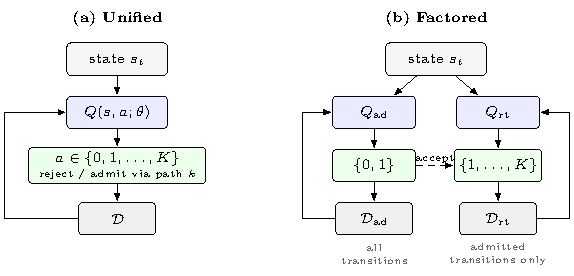
\includegraphics[width=\columnwidth]{fig_architecture.pdf}
\caption{Agent architectures. The unified agent (a) couples admission and
routing in one action space of size $K+1$ served by a single network and
replay buffer. The factored agent (b) uses independent estimators; the
routing network is queried only on accept and trained from a dedicated
buffer receiving admitted transitions only.}
\label{fig:arch}
\end{figure}

\subsection{Value Decomposition and Learning Rule}
%-----------------------------------------------------------------------
% [A-P2] GUIDANCE: Duelling decomposition and double-DQN target, briefly.
% State the two implementation choices that mattered: Huber loss with
% gradient clipping, and target sync every C environment STEPS (not
% episodes). Note ALL agents and baselines share these, so comparisons
% isolate architecture rather than training stability.
%-----------------------------------------------------------------------
Each network decomposes its output into value and advantage streams,
\begin{align}
Q(s,a;\theta,\alpha,\beta) &= V(s;\beta) \notag\\
&\quad + \Bigl( A(s,a;\alpha) - \tfrac{1}{|\mathcal{A}|}\textstyle\sum_{a'} A(s,a';\alpha) \Bigr),
\label{eq:duel}
\end{align}
and is trained on the double-DQN target
\begin{equation}
y_i = r_i + \gamma(1-\text{done}_i)\,
Q\bigl(s'_i,\ \arg\max_{a'} Q(s'_i,a';\theta);\ \theta^{-}\bigr),
\label{eq:target}
\end{equation}
minimising the Huber loss
\begin{equation}
L(\theta) = \mathbb{E}_{B\sim\mathcal{D}}
\Bigl[ \tfrac{1}{|B|}\sum_{i\in B} \mathcal{L}_{\delta}\bigl(y_i - Q(s_i,a_i;\theta)\bigr) \Bigr].
\label{eq:loss}
\end{equation}
Gradient norms are clipped and target parameters synchronised every $C$
environment steps. Every learned agent and every learned baseline shares
this loss, clipping and schedule, so comparisons reflect architecture and
representation rather than differences in training stability.

\subsection{The Factored Agent and the Routing Buffer}
%-----------------------------------------------------------------------
% [A-P3] GUIDANCE: The detail that makes the factored agent correct, and
% that explains its behaviour at rho=0. The routing network must train
% ONLY on admitted transitions -- a rejection exercises no path and
% carries no evidence about which path would have been better. Hence two
% buffers. Note the consequence that matters later: the admission
% estimator stays size-2 and sees every transition, i.e. structurally the
% SAME learning problem the admission-only baseline solves.
%-----------------------------------------------------------------------
In the factored agent the estimators learn from different experience
streams. The admission network learns from every transition, since both
accepting and rejecting are informative. The routing network learns only
from transitions in which a slice was admitted: a rejected request
exercises no path and carries no evidence about which path would have been
preferable. The agent therefore maintains $\mathcal{D}_{\text{ad}}$,
receiving all transitions, and $\mathcal{D}_{\text{rt}}$, receiving
admitted transitions only. One consequence matters for
Section~\ref{sec:architecture}: the admission estimator remains a size-two
head trained on every transition, which is structurally the same learning
problem the admission-only baseline solves.

\begin{algorithm}[t]
\caption{Training loop for both architectures}
\label{alg:training}
\scriptsize
\begin{algorithmic}[1]
\State \textbf{Input:} topology $G$, episodes $M$, steps $T$
\If{\texttt{unified}}
    \State initialise $Q(\cdot;\theta)$, target $\hat{Q}$, buffer $\mathcal{D}$
\Else
    \State initialise $Q_{\text{ad}},Q_{\text{rt}}$ and targets; buffers $\mathcal{D}_{\text{ad}},\mathcal{D}_{\text{rt}}$
\EndIf
\State $n \gets 0$
\For{episode $=1$ to $M$}
  \State reset environment, observe $s_0$
  \For{$t=1$ to $T$}
    \State compute $\boldsymbol{\phi}$ from $\mathbf{B},\mathbf{M}_t,b_t$ \Comment{Eq.~\eqref{eq:phi}}
    \If{\texttt{unified}}
        \State $a_t \gets \epsilon\text{-greedy}(Q(s_t,\cdot))$
    \Else
        \State $a^{\text{ad}} \gets \epsilon\text{-greedy}(Q_{\text{ad}}(s_t,\cdot))$
        \If{$a^{\text{ad}}=1$} $a^{\text{rt}} \gets \epsilon\text{-greedy}(Q_{\text{rt}}(s_t,\cdot))$
        \Else\ $a^{\text{rt}} \gets \varnothing$ \EndIf
    \EndIf
    \State execute (Algorithm~\ref{alg:step}); observe $r_t,s_{t+1}$
    \If{\texttt{unified}} push to $\mathcal{D}$
    \Else\ push to $\mathcal{D}_{\text{ad}}$; \textbf{if} $a^{\text{ad}}=1$ push to $\mathcal{D}_{\text{rt}}$
    \EndIf
    \State sample mini-batch(es); targets by~\eqref{eq:target}; minimise~\eqref{eq:loss}
    \State $n \gets n+1$; \textbf{if} $n \bmod C = 0$ synchronise targets
  \EndFor
\EndFor
\end{algorithmic}
\end{algorithm}

\begin{algorithm}[t]
\caption{Environment step: admission and reservation}
\label{alg:step}
\scriptsize
\begin{algorithmic}[1]
\State \textbf{Input:} request $r_t$, action (reject, or admit via path $k$)
\If{action is reject} \textbf{return} reward $0$ \EndIf
\State $\mathcal{C} \gets \{(i,j) : \mathbf{M}_t(i,j)=1\}$
\ForAll{$(i,j) \in \mathcal{C}$} \Comment{verify ALL before reserving ANY}
   \State $P_{i,j} \gets k$-th path of $\mathcal{P}_{i,j}$
   \If{$P_{i,j}$ undefined \textbf{or} $\min_{e \in P_{i,j}} A_e < b_t$}
       \State \textbf{return} reward $0$ \Comment{attempt fails; nothing reserved}
   \EndIf
\EndFor
\ForAll{$(i,j) \in \mathcal{C}$} $A_e \gets A_e - b_t,\ \forall e \in P_{i,j}$ \EndFor
\State register slice with lifetime $d_t$; \textbf{return} reward $1$
\State \textbf{on expiry:} $A_e \gets A_e + b_t$ for every reserved link
\end{algorithmic}
\end{algorithm}

%-----------------------------------------------------------------------
% [A-P4] GUIDANCE: One paragraph on Algorithm 2: the two-pass structure
% verifies ALL required connections before reserving ANY, so a slice is
% never partially embedded -- this is what guarantees fulfilment = 1.
%-----------------------------------------------------------------------
Algorithm~\ref{alg:step} details the transition. Its two-pass structure
matters: every required connection is verified against residual capacity
before any reservation is made, so a slice is never partially embedded.
With capacity released on expiry, this guarantees that every admitted
slice is served at its requested rate throughout its lifetime.

%=======================================================================
\section{Simulation Framework and Protocol} \label{expSetup}
%=======================================================================

\subsection{Framework}
%-----------------------------------------------------------------------
% [E-P1] GUIDANCE: Describe honestly. Flow-level discrete-event simulator
% implementing the Gymnasium API, agents in PyTorch, containerised for
% reproducible GPU runs. One step = one slice arrival. An Open vSwitch
% interface instantiates computed embeddings on an emulated data plane
% and is used to verify they correspond to realisable forwarding state.
% BE PRECISE: all reported numbers come from the flow-level simulator.
% Do NOT claim packet-level measurements -- none were made.
%-----------------------------------------------------------------------
Experiments run in a flow-level discrete-event simulator implementing the
Gymnasium API, with agents in PyTorch and the stack containerised for
reproducible execution on GPU servers. One simulation step corresponds to
one slice arrival; lifetimes are decremented each step and capacity
returned on expiry. An Open vSwitch interface allows embeddings produced
by a trained policy to be instantiated on an emulated data plane, which we
use to verify that computed reservations correspond to realisable
forwarding state. All performance figures reported here are obtained from
the flow-level simulator.

\subsection{Substrates}
%-----------------------------------------------------------------------
% [E-P2] GUIDANCE: Describe the operator topology, the Waxman substrate,
% and the controlled rho family. Emphasise the family's design: ONE fixed
% core graph, same endpoints and traffic, varying ONLY the access/core
% capacity ratio, with capacity_scale calibrated per level so greedy
% acceptance is ~0.47 everywhere. Explain WHY that calibration is
% essential: the advantage is load dependent (Sec VI-F), so without it
% rho would be confounded with offered load. Reference
% Table~\ref{tab:topologies} and Table~\ref{tab:rhofamily}.
%-----------------------------------------------------------------------
Three substrate sets are used. The first is a real operator topology with
$86$ nodes of which $21$ are slice endpoints. The second is deliberately
dissimilar: a synthetic graph with a Waxman random-geometric core, fewer
endpoints, a different degree distribution and heterogeneous capacities.
Their characteristics are in Table~\ref{tab:topologies}; critically they
are matched in the difficulty they present to an admission controller,
both admitting roughly $47\%$ of arrivals under greedy, yet differ almost
maximally in $\rho$.

The third is a controlled family built to test the hypothesis of
Section~\ref{model} directly. It uses one fixed core graph, the same
endpoint count and attachment, and the same traffic process, and varies
only the access-to-core capacity ratio -- the quantity shown above to
determine $\rho$. Because the advantage of joint control is itself load
dependent (Section~\ref{sec:load}), each member is calibrated by binary
search on a global capacity scale so that greedy acceptance is
approximately $0.47$ at every level. Without that calibration $\rho$ would
be confounded with offered load and the sweep would establish nothing.
Table~\ref{tab:rhofamily} reports the resulting family: $\rho$ spans
$0$ to $14.4\%$ while greedy acceptance stays within one percentage point.

\begin{table}[t]
\centering
\caption{Characteristics of the two evaluation substrates.}
\label{tab:topologies}
\renewcommand{\arraystretch}{1.15}
\begin{tabular}{lcc}
\toprule
& \textbf{Operator} & \textbf{Waxman} \\
\midrule
Total nodes                        & $86$    & $39$ \\
Endpoint nodes $|V_a|$             & $21$    & $15$ \\
Links                              & $106$   & $71$ \\
Access / core capacity ratio       & $2.00$  & $0.41$ \\
Endpoint pairs with $\geq 3$ paths & $96.7\%$ & $100\%$ \\
State dimension \eqref{eq:statedim}, $K{=}3$ & $1773$ & $909$ \\
Greedy acceptance                  & $0.4637$ & $0.4683$ \\
Routing headroom $\rho$            & $\mathbf{11.0\%}$ & $\mathbf{0.0\%}$ \\
\bottomrule
\end{tabular}
\end{table}

\begin{table}[t]
\centering
\caption{The controlled $\rho$ family. One fixed core graph; only the
access/core capacity ratio varies. The capacity scale is calibrated per
level so that greedy acceptance is held fixed, decoupling $\rho$ from
offered load.}
\label{tab:rhofamily}
\renewcommand{\arraystretch}{1.15}
\begin{tabular}{cccc}
\toprule
\textbf{Access/core ratio} & \textbf{Capacity scale} & \textbf{Greedy acc.} & $\boldsymbol{\rho}$ \\
\midrule
$0.4$ & $1.795$ & $0.4783$ & $0.00\%$ \\
$0.8$ & $0.904$ & $0.4739$ & $0.70\%$ \\
$1.3$ & $0.561$ & $0.4785$ & $5.08\%$ \\
$2.0$ & $0.390$ & $0.4838$ & $12.91\%$ \\
$3.0$ & $0.344$ & $0.4744$ & $14.42\%$ \\
\bottomrule
\end{tabular}
\end{table}

\subsection{Traffic, Baselines and Protocol}
%-----------------------------------------------------------------------
% [E-P3] GUIDANCE: Traffic model in 2 sentences, pointing at
% Table~\ref{tab:hyper}.
%-----------------------------------------------------------------------
Slice requests arrive as a Poisson process with geometrically distributed
lifetimes, uniform bandwidth demands, and one to three logical connections
between randomly chosen endpoints, with inelastic and elastic types
equally likely. Values are in Table~\ref{tab:hyper}.

%-----------------------------------------------------------------------
% [E-P4] GUIDANCE: The four baselines. Be explicit that greedy is STRONG,
% not a straw man: admits every feasible request, picks the max-bottleneck
% path, never routing-errors -> optimal among memoryless policies. This
% protects the modest greedy margin from looking like a weak-comparator
% artefact. Then revenue threshold, AC-only, and the aggregate-state DQN.
%-----------------------------------------------------------------------
Four baselines are used. \emph{Greedy} admits every request for which at
least one candidate path is feasible and routes it over the path with the
largest residual bottleneck. It is deliberately strong: capacity-aware,
routing-aware, never rejecting a request it could serve and never
selecting an infeasible path. It is optimal among memoryless policies, so
any improvement over it must come from foresight rather than from better
instantaneous decisions. \emph{Revenue threshold} admits only when
$d_t p_t$ exceeds a calibrated threshold, routing over the shortest path.
\emph{AC-only DQN} learns admission with the same network, loss and
schedule as the joint agents but always routes over the shortest path,
isolating the contribution of learned routing.

%-----------------------------------------------------------------------
% [E-P5] GUIDANCE: The fourth baseline and WHY it is constructed this
% way. Published 5G-core methods target different substrates and
% objectives, so a verbatim port would compare problems rather than
% methods. We reproduce the methodological essence -- aggregate resource
% state, no path-level routing -- while holding objective, algorithm,
% loss, schedules and budget identical. Stress the fairness point: it
% optimises the SAME count objective, so it is not beaten on a metric it
% never targeted. Say what it isolates: vs AC-only (full state, also
% cannot route) it isolates the path-level STATE; vs the joint agent,
% state and routing together.
%-----------------------------------------------------------------------
The fourth baseline represents the published 5G-core literature. Methods
such as SARA/DSARA~\cite{villota2022admission}, FSAC~\cite{wang2024fsac}
and the online formulation of~\cite{sulaiman2025datadriven} share two
structural properties: the substrate is described as aggregate resource
pools rather than per-pair, per-path state, and routing is not in the
action space. Porting any of them verbatim is not meaningful here, since
each targets a different substrate and objective, so the result would
compare problems rather than methods. We therefore reproduce the
methodological essence. \emph{Aggregate-state DQN} observes only the
request features, the active-slice counts and four scalar summaries of
residual capacity -- mean, minimum, dispersion and the fraction of paths
too small for the request -- with no per-pair resolution and no
feasibility signal, and decides admission alone, routing over the shortest
path. Everything else is identical to our agents: the same count
objective, duelling architecture, loss, clipping, exploration schedule and
training budget. The comparison is therefore one of representation rather
than of objectives. Measured against AC-only, which sees the full state
but also cannot route, it isolates the value of the path-level state;
measured against the joint agent it isolates state and routing together.

%-----------------------------------------------------------------------
% [E-P6] GUIDANCE: Metrics and statistics -- this is what makes small
% margins defensible. Acceptance ratio is the metric (fulfilment is
% identically 1). Five training seeds for principal comparisons, two or
% three for secondary. Every policy evaluated with exploration disabled
% on held-out traffic from a disjoint seed, 200 episodes (~1e5 arrivals).
% Within a seed all policies see the SAME traffic, so comparisons are
% PAIRED; report paired t-tests. Explain why pairing matters: it removes
% traffic variance and is far more powerful at this sample size.
%-----------------------------------------------------------------------
The reported metric is the acceptance ratio; as established in
Section~\ref{model} the fulfilment ratio is identically one. Each
configuration is trained with five independent seeds for the principal
comparisons and two or three for the secondary studies. Every trained
policy is evaluated with exploration disabled on held-out traffic
generated from a disjoint seed, for $200$ episodes, approximately $10^5$
arrivals. Within a seed all policies see identical traffic, so comparisons
are paired and we report paired $t$-tests across seeds. Pairing removes
between-seed traffic variance and is substantially more powerful than
comparing independent means at this sample size, which matters because
several of the effects are small. Comparisons that do not reach
significance are marked as such throughout.

\begin{table}[t]
\centering
\caption{Environment and training parameters.}
\label{tab:hyper}
\renewcommand{\arraystretch}{1.12}
\begin{tabular}{lc}
\toprule
\textbf{Parameter} & \textbf{Value} \\
\midrule
Candidate paths $K$              & $3$ (also $6$, $8$) \\
Arrival rate $\lambda$           & $5.0$ \\
Mean slice lifetime              & $30$ \\
Bandwidth demand                 & $\mathcal{U}[10,100]$ Mb/s \\
Logical connections per request  & $\mathcal{U}\{1,2,3\}$ \\
$\Pr[\text{inelastic}]$          & $0.5$ \\
\midrule
Episodes / steps per episode     & $2000$ / $500$ \\
Discount $\gamma$                & $0.99$ \\
Learning rate                    & $10^{-4}$ \\
Hidden units                     & $256$ \\
Mini-batch size                  & $64$ \\
Replay capacity                  & $5\times10^{4}$ \\
$\epsilon$: start $\to$ end      & $1.0 \to 0.05$ \\
$\epsilon$ decay steps           & $2\times10^{5}$ \\
Target sync interval $C$ (steps) & $100$ \\
Training seeds                   & $42$--$46$ \\
Evaluation                       & held-out seed, $200$ episodes, $\epsilon=0$ \\
\bottomrule
\end{tabular}
\end{table}

%=======================================================================
\section{Results} \label{results}
%=======================================================================

\subsection{Acceptance on the Operator Substrate}
\label{sec:main}
%-----------------------------------------------------------------------
% [R-P1] GUIDANCE: Table~\ref{tab:main} and Fig.~\ref{fig:main}.
% Numbers: joint 0.4806+-0.0043; factored 0.4739+-0.0049; greedy
% 0.4637+-0.0028; AC-only 0.4476+-0.0022; aggregate 0.4195+-0.0012;
% revenue 0.1308. Paired vs joint: greedy +3.6% (t=7.44), AC-only +7.4%
% (t=11.60), aggregate +14.55% (t=28.21), revenue +267.5%.
% Tone: state plainly; do NOT oversell the 3.6%.
%-----------------------------------------------------------------------
Table~\ref{tab:main} and Fig.~\ref{fig:main} report acceptance on the
operator substrate with $K=3$. The joint unified agent admits $48.06\%$ of
arrivals against $46.37\%$ for greedy, an improvement of $3.6\%$
consistent across all five seeds and significant under a paired test
($t=7.44$). The margin over the admission-only agent is $7.4\%$, and over
the aggregate-state controller representing the published literature it is
$14.6\%$.

%-----------------------------------------------------------------------
% [R-P2] GUIDANCE: Interpret the margins honestly and pre-empt the
% obvious criticism. Greedy is optimal among memoryless policies, so
% +3.6% is the value of FORESIGHT alone, not of "ML over heuristics".
% Then the decomposition the aggregate baseline enables -- this is the
% paragraph that makes the baseline worth having:
%   AC-only (full state, no routing) vs aggregate (aggregate state, no
%   routing) = +6.7% -> the value of the path-level STATE alone;
%   joint vs aggregate = +14.6% -> state AND routing together.
% Also note the aggregate controller is beaten by greedy itself
% (-10.5%), i.e. an aggregate-resource learned policy underperforms a
% simple bottleneck-aware heuristic on a path-level substrate.
%-----------------------------------------------------------------------
The magnitudes deserve comment. Greedy never declines a request it could
serve and never chooses an infeasible path, so it is optimal among
policies without memory; the $3.6\%$ improvement is therefore attributable
entirely to foresight, not to replacing a heuristic with a learned policy.
The aggregate-state baseline permits a sharper decomposition. It differs
from the AC-only agent only in its state representation, since neither can
route, and that difference alone is worth $6.7\%$. Adding routing takes the
total to $14.6\%$. Notably the aggregate-state controller is itself
outperformed by greedy, by $10.5\%$: on a substrate where capacity is
distributed across paths, a learned policy that observes only aggregate
resources is worse than a simple bottleneck-aware heuristic.

\begin{table}[t]
\centering
\caption{Acceptance on the operator substrate ($K=3$, five seeds,
held-out evaluation). Paired statistics against the unified joint agent.}
\label{tab:main}
\renewcommand{\arraystretch}{1.2}
\begin{tabular}{lccc}
\toprule
\textbf{Policy} & \textbf{Acceptance} & \textbf{$\Delta$ vs.\ joint} & \textbf{Paired $t$} \\
\midrule
Joint, unified      & $\mathbf{0.4806 \pm 0.0043}$ & --- & --- \\
Joint, factored     & $0.4739 \pm 0.0049$ & $-1.4\%$ & $-2.13$ (n.s.) \\
Greedy              & $0.4637 \pm 0.0028$ & $-3.6\%$ & $7.44^{*}$ \\
AC-only DQN         & $0.4476 \pm 0.0022$ & $-7.4\%$ & $11.60^{*}$ \\
Aggregate-state DQN & $0.4195 \pm 0.0012$ & $-14.6\%$ & $28.21^{*}$ \\
Revenue threshold   & $0.1308 \pm 0.0011$ & $-267.5\%$ & $187.11^{*}$ \\
\bottomrule
\multicolumn{4}{l}{\footnotesize $^{*}$ significant at $\alpha=0.05$ ($t_{\text{crit}}=2.776$, $\mathrm{df}=4$).}
\end{tabular}
\end{table}

\begin{figure}[t]
\centering
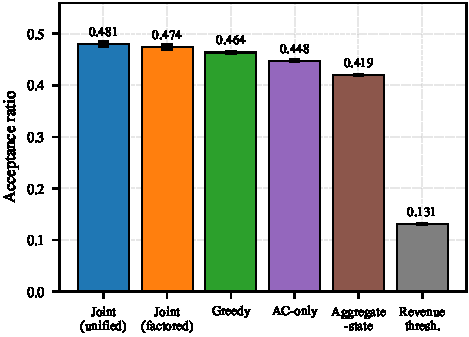
\includegraphics[width=\columnwidth]{fig_main.pdf}
\caption{Acceptance on the operator substrate ($K=3$, mean and standard
deviation over five seeds). The aggregate-state controller, representing
the published 5G-core state abstraction, is outperformed even by greedy.}
\label{fig:main}
\end{figure}

%-----------------------------------------------------------------------
% [R-P3] GUIDANCE: Learning curves, Fig.~\ref{fig:learning}. The factored
% agent is slower early because its routing estimator only sees admitted
% transitions and so accumulates experience more slowly; both converge
% without instability. Note curves are training-window averages with
% exploration active, so they sit below the held-out numbers.
%-----------------------------------------------------------------------
Fig.~\ref{fig:learning} shows training progression. The factored agent
improves more slowly early on, as expected: its routing estimator receives
only transitions in which a slice was admitted and so accumulates usable
experience at a fraction of the rate of the admission estimator. Both
converge without instability. The curves are training-window averages with
exploration still active and therefore lie below the held-out values of
Table~\ref{tab:main}.

\begin{figure}[t]
\centering
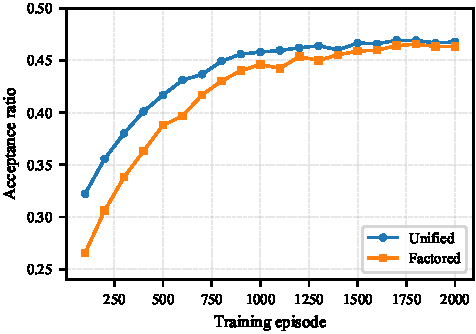
\includegraphics[width=\columnwidth]{fig_learning.pdf}
\caption{Training progression on the operator substrate (seed $42$).}
\label{fig:learning}
\end{figure}

\subsection{What the Agent Learns: Admissibility Preservation}
\label{sec:mechanism}
%-----------------------------------------------------------------------
% [R-P4] GUIDANCE: The mechanism. Set up the question: why does a policy
% beat one that never refuses a feasible request? Answer: it declines
% admissible requests to keep the substrate routable. Introduce the
% measurement and stress it is ENDOGENOUS -- measured along each policy's
% OWN trajectory, so it reflects the capacity that policy has committed.
%-----------------------------------------------------------------------
Greedy never declines a request it could serve, so an agent admitting more
than greedy must be creating admission opportunities that would not
otherwise exist. To identify the mechanism we measure, along each policy's
own trajectory, the fraction of arrivals for which at least one candidate
path is feasible. The quantity is endogenous: it is determined by the
capacity the policy has already committed, and so measures the extent to
which a policy has preserved its own future freedom of action.

%-----------------------------------------------------------------------
% [R-P5] GUIDANCE: Table~\ref{tab:mechanism} and
% Fig.~\ref{fig:feasibility}. Operator: 54.89% vs 46.19% (+8.70pp);
% Waxman: 53.27% vs 46.68% (+6.59pp). Interpretation: by declining a
% minority of admissible requests -- typically those whose embedding
% would consume scarce shared links -- the agent keeps the substrate in a
% state where a larger share of FUTURE arrivals can be served, and admits
% more in total. This is non-myopic behaviour unavailable to a memoryless
% policy, and it is why the margin in Table~\ref{tab:main} exists.
%-----------------------------------------------------------------------
Table~\ref{tab:mechanism} and Fig.~\ref{fig:feasibility} report the
result. On the operator substrate the learned policy sustains $54.89\%$
feasible arrivals against $46.19\%$ under greedy, a difference of $8.7$
percentage points, and the effect reappears on the Waxman substrate at
$53.27\%$ against $46.68\%$. The interpretation is direct: by declining a
minority of admissible requests -- characteristically those whose
embedding would consume capacity on heavily shared links -- the agent
keeps the substrate in a state where a larger fraction of subsequent
arrivals can still be served, and admits more slices in aggregate. This is
precisely the behaviour a memoryless policy cannot exhibit, and it is why
the margin of Table~\ref{tab:main} exists.

\begin{table}[t]
\centering
\caption{Decision decomposition and admissibility preservation (three
seeds). Feasible arrivals are measured along each policy's own trajectory.}
\label{tab:mechanism}
\renewcommand{\arraystretch}{1.2}
\begin{tabular}{lcc}
\toprule
& \textbf{Operator} & \textbf{Waxman} \\
\midrule
Feasible arrivals, learned policy & $54.89\%$ & $53.27\%$ \\
Feasible arrivals, greedy         & $46.19\%$ & $46.68\%$ \\
\textbf{Preservation gain}        & $\mathbf{+8.70}$ pp & $\mathbf{+6.59}$ pp \\
\midrule
Admitted                          & $47.06\%$ & $48.50\%$ \\
Routing errors                    & $4.60\%$  & $\mathbf{0.00\%}$ \\
Missed admissions                 & $3.23\%$  & $4.77\%$ \\
\bottomrule
\end{tabular}
\end{table}

\begin{figure}[t]
\centering
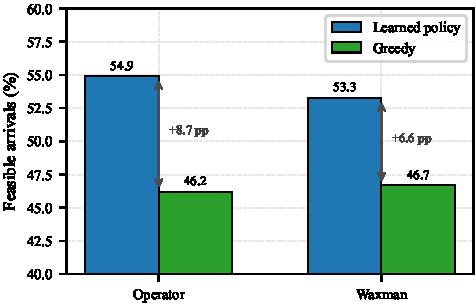
\includegraphics[width=\columnwidth]{fig_feasibility.pdf}
\caption{Admissibility preservation. The learned policy keeps a
substantially larger fraction of future arrivals routable than greedy on
both substrates.}
\label{fig:feasibility}
\end{figure}

%-----------------------------------------------------------------------
% [R-P6] GUIDANCE: Use the last rows of Table~\ref{tab:mechanism} twice.
% (a) Bound the headroom honestly: on the operator substrate 4.60%
% routing errors + 3.23% missed admissions means ~7.8pp of the agent's
% own opportunity is unexploited, so the policy is not optimal; forward
% ref Sec~\ref{sec:ablations} where masking fails to recover it.
% (b) MORE IMPORTANT: routing errors are 4.60% on the operator substrate
% and exactly 0.00% on the Waxman one. That is the first direct evidence
% that the routing decision is pivotal on one substrate and inert on the
% other -- it motivates the law in the next subsection.
%-----------------------------------------------------------------------
Two further observations follow. The learned policy still attempts
admission on an infeasible path in $4.60\%$ of arrivals and declines a
feasible request in a further $3.23\%$, so close to eight percentage
points of the opportunity it creates go unused: the policy is clearly
suboptimal, and Section~\ref{sec:ablations} shows this residue is not
trivially recoverable. More consequentially, the routing-error rate is
$4.60\%$ on the operator substrate and exactly $0.00\%$ on the Waxman one.
On the latter the agent never selects an infeasible path when a feasible
one exists -- not because it routes well, but because the shortest path is
feasible whenever any path is. This is the first direct evidence that the
routing decision is pivotal on one substrate and inert on the other, and
it motivates the law we establish next.

\subsection{The Routing-Headroom Law}
\label{sec:law}
%-----------------------------------------------------------------------
% [R-P7] GUIDANCE: THE central result -- give it the most care in the
% paper. Set up: Sec VI-B showed routing is pivotal on one substrate and
% inert on another; rho (Def~\ref{def:rho}) quantifies that; the family
% of Table~\ref{tab:rhofamily} manipulates rho alone. Then the result
% from Table~\ref{tab:law} and Fig.~\ref{fig:rho}: the gap rises from
% -1.65% at rho=0.70% to +12.74% at rho=14.42%, linear with r^2=0.979,
% slope ~0.97 (each point of rho buys ~1% relative advantage), sign
% change near rho=2%.
%-----------------------------------------------------------------------
Section~\ref{sec:mechanism} established that the routing decision is
pivotal on one substrate and inert on another. The routing headroom $\rho$
of Definition~\ref{def:rho} quantifies exactly that, and the family of
Table~\ref{tab:rhofamily} manipulates it while holding the operating point
fixed. Table~\ref{tab:law} and Fig.~\ref{fig:rho} report the outcome. The
advantage of joint control over admission-only control rises
monotonically in $\rho$ across the range tested, from $-1.65\%$ where
routing is nearly useless to $+12.74\%$ where it is most valuable, and the
relationship is close to linear, with $r^2=0.979$. The fitted slope is
approximately $0.97$, so each percentage point of routing headroom buys
roughly one percent of relative advantage, and the gap changes sign near
$\rho \approx 2\%$.

%-----------------------------------------------------------------------
% [R-P8] GUIDANCE: The MECHANISM behind the law -- read the columns of
% Table~\ref{tab:law} / panel (a) of Fig.~\ref{fig:rho}. The gap widens
% because AC-only FALLS (0.4934 -> 0.4236 as rho grows), not because the
% joint agent rises (0.4906 -> 0.4776, essentially flat). As more
% arrivals are admissible only off the shortest path, the fixed-path
% controller progressively loses reach while the joint agent retains it.
% Greedy is also flat, as expected since it selects the best path. This
% is important: the law is not a curve fit, it has a mechanism.
%-----------------------------------------------------------------------
The mechanism is visible in the columns. The gap widens not because the
joint agent improves -- its acceptance is essentially flat across the
family, from $0.4906$ to $0.4776$ -- but because the admission-only
controller deteriorates, from $0.4934$ to $0.4236$. As a growing fraction
of arrivals becomes admissible only off the shortest path, a controller
pinned to that path progressively loses reach, while one able to choose
retains it. Greedy, which also selects among paths, is likewise flat. The
law therefore has a mechanical explanation rather than being an empirical
fit: $\rho$ measures the reach that a fixed-path policy forfeits.

%-----------------------------------------------------------------------
% [R-P9] GUIDANCE: Out-of-family validation and the deployment rule.
% The two real substrates were NOT part of the family and were built by
% different processes, yet both sit close to the fitted line (operator
% rho=11.0%, gap +7.4%; Waxman rho=0.0%, gap -2.3%) -- shown as diamonds
% in Fig.~\ref{fig:rho}(b). Then state the operational rule: measure the
% access/core provisioning ratio, obtain rho, and decide the architecture
% BEFORE training anything. Note the asymmetry: deploying joint control
% where rho=0 cost 2.3% of acceptance here.
%-----------------------------------------------------------------------
The two real substrates provide out-of-family validation. Neither was part
of the calibrated family and both were produced by different construction
processes, yet each falls close to the fitted line: the operator topology
at $\rho=11.0\%$ with a measured gap of $+7.4\%$, and the Waxman substrate
at $\rho=0.0\%$ with $-2.3\%$. These are the diamonds in
Fig.~\ref{fig:rho}(b). The practical consequence is a rule requiring no
training: estimate the access-to-core provisioning ratio of the intended
substrate, obtain $\rho$ from it, and choose the architecture before
committing to it. The asymmetry matters, since deploying joint control
where routing is useless cost $2.3\%$ of acceptance in our measurements.

\begin{table}[t]
\centering
\caption{The routing-headroom law. Acceptance of each policy across the
controlled family (two seeds per level), and the resulting advantage of
joint over admission-only control.}
\label{tab:law}
\renewcommand{\arraystretch}{1.2}
\begin{tabular}{ccccc}
\toprule
$\boldsymbol{\rho}$ & \textbf{Joint} & \textbf{Greedy} & \textbf{AC-only} & \textbf{Joint $-$ AC-only} \\
\midrule
$0.00\%$  & $0.4906$ & $0.4708$ & $0.4934$ & $-0.58\%$ \\
$0.70\%$  & $0.4829$ & $0.4740$ & $0.4910$ & $-1.65\%$ \\
$5.08\%$  & $0.4820$ & $0.4788$ & $0.4728$ & $+1.96\%$ \\
$12.91\%$ & $0.4843$ & $0.4849$ & $0.4386$ & $+10.43\%$ \\
$14.42\%$ & $0.4776$ & $0.4774$ & $0.4236$ & $+12.74\%$ \\
\midrule
\multicolumn{5}{l}{\footnotesize Least-squares fit: $\text{gap} = 0.97\rho - 1.82$, $r^2 = 0.979$.} \\
\bottomrule
\end{tabular}
\end{table}

\begin{figure*}[t]
\centering
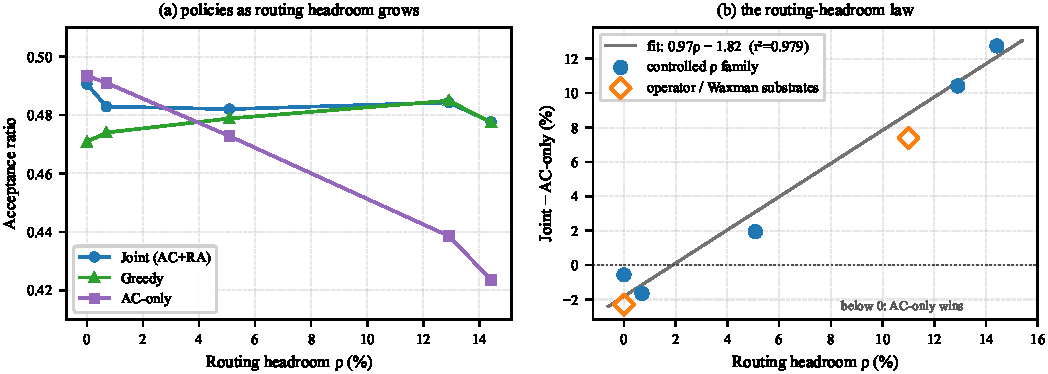
\includegraphics[width=\textwidth]{fig_rho.pdf}
\caption{The routing-headroom law. (a) As $\rho$ grows the
admission-only controller loses reach while the joint agent and greedy,
both able to select among paths, remain flat. (b) The resulting advantage
of joint over admission-only control is linear in $\rho$ ($r^2=0.979$) and
changes sign near $\rho\approx2\%$. Diamonds mark the two real substrates,
which were not part of the calibrated family.}
\label{fig:rho}
\end{figure*}

\subsection{Which Architecture to Deploy}
\label{sec:architecture}
%-----------------------------------------------------------------------
% [R-P10] GUIDANCE: The law implies a substrate-dependent CHOICE, which
% is awkward operationally. This subsection shows the choice can be
% avoided. Set up with Table~\ref{tab:topo2}/Fig.~\ref{fig:topo2}: on the
% rho=0 substrate the UNIFIED joint agent is significantly worse than
% AC-only (0.4858 vs 0.4970, +2.30%, t=5.97, 5/5). Note the measured
% routing_error there is 0.00%, so the deficit is NOT bad routing.
%-----------------------------------------------------------------------
Taken alone the law implies a substrate-dependent choice of architecture,
which is awkward operationally. This subsection shows the choice can be
avoided. Table~\ref{tab:topo2} and Fig.~\ref{fig:topo2} report the
$\rho=0$ substrate in full. The unified joint agent admits $48.58\%$
against $49.70\%$ for the admission-only controller, a deficit of
$2.30\%$ that is consistent across all five seeds and significant
($t=5.97$). As Section~\ref{sec:mechanism} showed, its routing-error rate
on this substrate is $0.00\%$, so the deficit is not caused by poor
routing.

%-----------------------------------------------------------------------
% [R-P11] GUIDANCE: The explanation and the fix. Explanation: with K+1
% actions, three of which are near-identical when rho=0, experience is
% spread across them and the admit-vs-reject boundary is estimated less
% sharply; the admission-only controller concentrates all experience on
% two actions. The factored agent's admission estimator is ALSO size-2
% and ALSO sees every transition (Sec~\ref{agents}), so it should not pay
% this cost. Result: factored 0.4930, beating unified by +1.49%
% (t=3.91, 5/5) and NOT significantly below AC-only (-0.79%, t=-1.72).
% BE PRECISE: "not significantly worse" is not "better".
%-----------------------------------------------------------------------
The explanation is estimation dilution. With $K+1$ actions, three of which
are near-indistinguishable when $\rho=0$, experience is divided among
them and the admit-versus-reject boundary is estimated less sharply, while
the admission-only controller concentrates all of its experience on two
actions. The factored agent should not pay this cost, because its
admission estimator is also a size-two head trained on every transition.
The measurements bear this out: it reaches $0.4930$, exceeding the unified
agent by $1.49\%$ ($t=3.91$, five seeds of five) and falling short of the
admission-only controller by only $0.79\%$, a difference that does not
reach significance ($t=-1.72$). We are careful here: not significantly
worse is not the same as better, and the factored agent's point estimate
on this substrate remains below the admission-only controller.

%-----------------------------------------------------------------------
% [R-P12] GUIDANCE: The recommendation. Combine both substrates: at
% rho=0 factored is statistically indistinguishable from AC-only; at
% rho=11% it beats AC-only by +5.9% (t=10.63). So the factored agent is
% never significantly worse and sometimes much better -- it dominates,
% and removes the need for a substrate-dependent choice. This is the
% paper's operational recommendation; state it plainly.
%-----------------------------------------------------------------------
Combining the two substrates yields the recommendation. Where $\rho=0$ the
factored agent is statistically indistinguishable from the admission-only
controller; where $\rho=11.0\%$ it exceeds it by $5.9\%$ ($t=10.63$). It is
therefore never significantly worse than the simpler design and
substantially better when routing matters. An operator who adopts the
factored architecture does not need to measure $\rho$ in order to choose,
although measuring it remains valuable for predicting how much the routing
component will contribute.

\begin{table}[t]
\centering
\caption{Acceptance on the $\rho=0$ substrate (five seeds). The ordering
reverses relative to Table~\ref{tab:main}: the admission-only controller
is the strongest policy, and the unified joint agent is significantly
worse than it.}
\label{tab:topo2}
\renewcommand{\arraystretch}{1.2}
\begin{tabular}{lccc}
\toprule
\textbf{Policy} & \textbf{Acceptance} & \textbf{$\Delta$ vs.\ unified} & \textbf{Paired $t$} \\
\midrule
AC-only DQN        & $\mathbf{0.4970 \pm 0.0044}$ & $+2.30\%$ & $5.97^{*}$ \\
Joint, factored    & $0.4930 \pm 0.0048$ & $+1.49\%$ & $3.91^{*}$ \\
Joint, unified     & $0.4858 \pm 0.0028$ & --- & --- \\
Greedy             & $0.4683 \pm 0.0026$ & $-3.74\%$ & $18.03^{*}$ \\
\midrule
\multicolumn{4}{l}{\footnotesize Factored vs.\ AC-only: $-0.79\%$, $t=-1.72$, not significant.} \\
\multicolumn{4}{l}{\footnotesize $^{*}$ significant at $\alpha=0.05$ ($t_{\text{crit}}=2.776$, $\mathrm{df}=4$).} \\
\bottomrule
\end{tabular}
\end{table}

\begin{figure}[t]
\centering
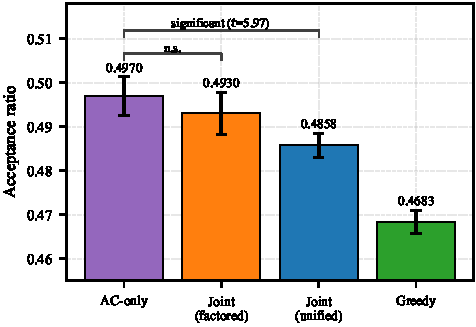
\includegraphics[width=\columnwidth]{fig_topo2.pdf}
\caption{Acceptance on the $\rho=0$ substrate. The unified joint agent is
significantly below the admission-only controller; the factored agent
recovers most of that deficit and is not significantly below it.}
\label{fig:topo2}
\end{figure}

\subsection{Scaling in the Number of Candidate Paths}
\label{sec:scaling}
%-----------------------------------------------------------------------
% [R-P13] GUIDANCE: Table~\ref{tab:scaling}/Fig.~\ref{fig:scaling}. At
% K=3 the architectures are indistinguishable (-1.4%, t=-2.13, n.s.);
% both flat at K=6; at K=8 unified falls to 0.4679 while factored holds
% at 0.4727. Unified degradation K=3->K=8 is -2.6% and significant
% (t=5.85); factored changes -0.3%, not significant. BE CAREFUL: the
% head-to-head at K=8 (+1.0%, 4/5 seeds, t=1.19) is NOT significant, so
% claim ROBUSTNESS (one architecture degrades, the other does not), NOT
% superiority.
%-----------------------------------------------------------------------
Table~\ref{tab:scaling} and Fig.~\ref{fig:scaling} compare the
architectures as the candidate path set grows. At $K=3$ they are
statistically indistinguishable, and both are flat at $K=6$. At $K=8$ they
separate: the unified agent falls to $0.4679$ while the factored agent
holds at $0.4727$. The unified degradation from $K=3$ to $K=8$ is $2.6\%$
and is significant ($t=5.85$), whereas the factored agent changes by
$0.3\%$, which is not. We are careful about what this supports: the
head-to-head difference at $K=8$ favours the factored agent on four seeds
of five but does not itself reach significance ($t=1.19$). The defensible
claim is robustness rather than superiority -- as the action space grows
the unified architecture degrades and the factored one does not.

%-----------------------------------------------------------------------
% [R-P14] GUIDANCE: Explain structurally and connect to Sec VI-D. In the
% unified formulation admission is inferred from a value estimate spread
% over K+1 entangled actions, so the admission problem itself gets harder
% as K rises -- the same estimation-dilution effect that produced the
% rho=0 deficit. The factored admission head stays size-2 for every K.
% So both results have ONE cause, which is a satisfying unification.
%-----------------------------------------------------------------------
The explanation is the one already encountered in
Section~\ref{sec:architecture}. In the unified formulation admission is
not represented separately: whether to admit must be inferred from a value
estimate spread over $K+1$ entangled actions, so the difficulty of the
admission problem itself grows with the number of paths offered. The
factored formulation keeps the admission estimator at two outputs for
every $K$ and widens only the routing estimator. The $\rho=0$ deficit and
the degradation with $K$ are therefore two symptoms of a single cause, and
both are avoided by the same architectural choice.

\begin{table}[t]
\centering
\caption{Acceptance versus the number of candidate paths $K$ (five seeds
at $K=3,8$; three at $K=6$).}
\label{tab:scaling}
\renewcommand{\arraystretch}{1.2}
\begin{tabular}{lccc}
\toprule
\textbf{Architecture} & $K=3$ & $K=6$ & $K=8$ \\
\midrule
Unified   & $0.4806 \pm 0.0043$ & $0.4802 \pm 0.0048$ & $0.4679 \pm 0.0071$ \\
Factored  & $0.4739 \pm 0.0049$ & $0.4752 \pm 0.0062$ & $0.4727 \pm 0.0040$ \\
\midrule
\multicolumn{4}{l}{\footnotesize Unified $K{=}3\to K{=}8$: $-2.6\%$ ($t=5.85$, significant).} \\
\multicolumn{4}{l}{\footnotesize Factored $K{=}3\to K{=}8$: $-0.3\%$ (not significant).} \\
\bottomrule
\end{tabular}
\end{table}

\begin{figure}[t]
\centering
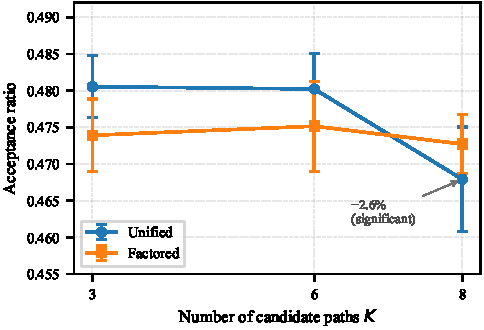
\includegraphics[width=\columnwidth]{fig_scaling.pdf}
\caption{Scaling in the number of candidate paths. The unified
architecture degrades significantly between $K=3$ and $K=8$; the factored
architecture is unaffected.}
\label{fig:scaling}
\end{figure}

\subsection{Sensitivity to Offered Load}
\label{sec:load}
%-----------------------------------------------------------------------
% [R-P15] GUIDANCE: Table~\ref{tab:load}/Fig.~\ref{fig:load}. At nominal
% load the joint margin over greedy is +3.6% (significant). Halving
% capacity drops acceptance to ~0.30 and the margin to +1.0%, consistent
% on 3/3 seeds but NOT significant (t=2.53, t_crit=4.303). The margin
% over AC-only is preserved (+5.5%, significant).
% INTERPRETATION: foresight needs SLACK to exploit. Under severe
% congestion nearly every feasible admission is forced and there is
% little scope to shape the future, so greedy approaches optimality. The
% method is therefore most valuable at moderate load -- which is the
% regime operators engineer for. This also explains why the rho family
% had to be calibrated to a fixed operating point.
%-----------------------------------------------------------------------
Table~\ref{tab:load} and Fig.~\ref{fig:load} examine offered load. Halving
the available capacity reduces acceptance for all policies to roughly
$0.30$ and the joint agent's margin over greedy falls from $3.6\%$ to
$1.0\%$; the direction is consistent across seeds but no longer
significant at this sample size. The margin over the admission-only agent
is preserved at $5.5\%$. The interpretation follows from the mechanism of
Section~\ref{sec:mechanism}: foresight requires slack to be exercised.
When capacity is severely constrained almost every feasible admission is
effectively forced and there is little scope to shape which requests
remain servable later, so greedy approaches optimality. The method is
consequently most valuable at moderate utilisation, which is the regime in
which transport networks are normally engineered to operate. This load
dependence is also why each member of the $\rho$ family had to be
calibrated to a common operating point.

\begin{table}[t]
\centering
\caption{Effect of offered load on the operator substrate (three seeds at
the high-load point).}
\label{tab:load}
\renewcommand{\arraystretch}{1.2}
\begin{tabular}{lcc}
\toprule
& \textbf{Nominal} & \textbf{High load} \\
\midrule
Joint, unified      & $0.4806$ & $0.3036 \pm 0.0013$ \\
Greedy              & $0.4637$ & $0.3006 \pm 0.0026$ \\
AC-only DQN         & $0.4476$ & $0.2878 \pm 0.0025$ \\
\midrule
Joint $-$ greedy    & $+3.6\%^{*}$ & $+1.0\%$ (n.s.) \\
Joint $-$ AC-only   & $+7.4\%^{*}$ & $+5.5\%^{*}$ \\
\bottomrule
\multicolumn{3}{l}{\footnotesize $^{*}$ significant at $\alpha=0.05$.}
\end{tabular}
\end{table}

\begin{figure}[t]
\centering
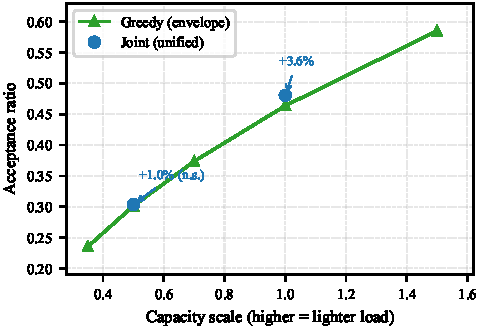
\includegraphics[width=\columnwidth]{fig_load.pdf}
\caption{Acceptance against offered load. The greedy curve traces the
operating envelope; the joint agent's advantage is largest at moderate
load and contracts under severe congestion.}
\label{fig:load}
\end{figure}

\subsection{Ablations and Negative Results}
\label{sec:ablations}
%-----------------------------------------------------------------------
% [R-P16] GUIDANCE: Action masking. Motivation: Sec VI-B showed 4.6% of
% arrivals lost to routing errors, and masking invalid actions is
% standard practice (cite huang2022invalid); phi identifies exactly which
% paths cannot serve the request. Result: it did NOT work. Masked
% 0.4602+-0.0208 vs unmasked 0.4806+-0.0043 -- mean falls 4.2% and the
% standard deviation grows FIVEFOLD, with two of five runs converging to
% visibly poorer policies. BE PRECISE: because variance explodes the mean
% difference is itself not significant (t=-2.09); the robust finding is
% the loss of STABILITY. Give the likely cause: the policy acts under the
% mask but the bootstrap target still maximises over unmasked actions, so
% behaviour and target policy are inconsistent. Report as a negative
% result for OUR implementation, not proof masking cannot work.
%-----------------------------------------------------------------------
Section~\ref{sec:mechanism} showed that $4.60\%$ of arrivals are lost to
routing errors, and the standard remedy is to mask invalid
actions~\cite{huang2022invalid}: the feasibility signal identifies exactly
which paths cannot serve the request. This did not work. With masking
enabled acceptance fell to $0.4602 \pm 0.0208$ from $0.4806 \pm 0.0043$,
and the more informative change is in the second moment, the standard
deviation across seeds growing roughly fivefold with two of five runs
converging to visibly poorer policies. Because of that variance the
difference in means is not itself significant ($t=-2.09$); the robust
finding is the loss of stability rather than of accuracy. The likely cause
is an inconsistency we did not correct: the behaviour policy selects among
masked actions while the bootstrap target in~\eqref{eq:target} still
maximises over the unmasked action set, so the agent learns towards a
policy it never executes. We report this as a negative result for our
implementation rather than as evidence that masking is inapplicable.

%-----------------------------------------------------------------------
% [R-P17] GUIDANCE: The revenue-objective ablation justifying Sec III-B.
% Under a revenue objective with soft capacity (over-admission permitted,
% SLA violations penalised) the agent DID beat greedy on the quantity it
% was given -- 222,239 vs 219,365 net revenue per episode -- but it did
% so by admitting FEWER slices than greedy in every regime tested. It
% wins the objective it is given, and that objective is not the one the
% slicing literature reports. Hence the count objective.
%-----------------------------------------------------------------------
We also examined the alternative revenue objective under a soft capacity
model permitting over-admission with penalised service-level violations.
Under that formulation the learned policy did outperform greedy on the
quantity it was asked to maximise, accruing $222{,}239$ against $219{,}365$
units of net revenue per episode, but it achieved this by admitting fewer
slices than greedy in every regime examined: it learned to prefer
expensive requests and decline inexpensive ones whose later violation
would cost more than they earn. The policy is correct for its objective,
but that objective is not the one under which slicing systems are
conventionally assessed, which motivated the count objective
of~\eqref{eq:objective}.

%=======================================================================
\section{Discussion} \label{discussion}
%=======================================================================
%-----------------------------------------------------------------------
% [D-P1] GUIDANCE: Separate robust from conditional -- this framing is
% the paper's main intellectual product. ROBUST across both substrates
% and both load regimes: learned non-myopic admission beats strong
% greedy, and the mechanism is admissibility preservation. CONDITIONAL,
% and we identify the governing quantity for each: the value of joint
% routing (governed by rho), the architecture choice (governed by K and
% by rho), and the size of the advantage (governed by load).
%-----------------------------------------------------------------------
It is worth separating what these experiments establish from what they
qualify. Two findings are robust across both substrates and both load
regimes: a learned admission policy outperforms a strong memoryless
heuristic, and it does so by preserving the admissibility of future
arrivals rather than by making better instantaneous decisions. Three
further findings are conditional, and for each we identified the governing
quantity: the value of learning routing jointly is governed by $\rho$, the
choice between unified and factored architectures is governed by the size
of the candidate path set and by $\rho$, and the magnitude of the
advantage is governed by offered load.

%-----------------------------------------------------------------------
% [D-P2] GUIDANCE: Operator-facing implications, three of them:
%  (i) the provisioning ratio already tells you rho, which tells you how
%      much routing will contribute -- all before training anything;
%  (ii) adopt the factored architecture: it is never significantly worse
%      and is robust to large K;
%  (iii) expect the benefit at moderate utilisation, not at saturation --
%      this is a capacity-planning aid, not a congestion remedy.
%-----------------------------------------------------------------------
Three implications follow for an operator. First, the access-to-core
provisioning ratio of the intended substrate already determines $\rho$,
which in turn predicts how much a routing component will contribute; both
can be evaluated before any agent is trained. Second, the factored
architecture should be adopted by default: it is never significantly worse
than the simpler admission-only design, it is substantially better where
routing matters, and it is robust as the candidate path set grows. Third,
the benefit should be expected at moderate utilisation rather than at
saturation; the method helps serve more slices from an adequately
provisioned network, and is not a remedy for a congested one.

%-----------------------------------------------------------------------
% [D-P3] GUIDANCE: Threats to validity -- state them plainly; reviewers
% respect it. (i) rho is validated on one controlled family plus two
% substrates, all with SINGLE-HOMED endpoints; multi-homed endpoints
% would break the structural argument that all candidate paths share the
% access links, and rho would then need re-deriving. (ii) the family uses
% two seeds per level, so the law rests on a trend across levels rather
% than on precision within a level. (iii) flow-level simulation: no
% queueing, transient congestion or packet effects. (iv) traffic is
% synthetic and stationary; real demand is correlated and
% non-stationary. (v) only value-based agents were studied.
%-----------------------------------------------------------------------
Several limitations qualify these conclusions. The law is validated on one
controlled family together with two independently constructed substrates,
all of which have single-homed endpoints; with multi-homed endpoints the
structural argument that every candidate path shares the same access links
no longer holds, and $\rho$ would have to be re-derived. The family uses
two seeds per level, so the law rests on the trend across levels rather
than on precision within any one of them. The evaluation is at flow level
and excludes queueing dynamics, transient congestion and packet-level
effects. The arrival process is synthetic and stationary, whereas real
slice demand is correlated and non-stationary. Finally only value-based
agents were examined; policy-gradient methods may behave differently,
particularly with respect to the masking result.

%-----------------------------------------------------------------------
% [D-P4] GUIDANCE: Future work, short and specific: (a) multi-homed
% endpoints, where rho must be redefined over per-path link sets;
% (b) correcting the masked-target inconsistency; (c) non-stationary
% demand and transfer across substrates, connecting to wang2024flagvne.
%-----------------------------------------------------------------------
Three extensions follow naturally. Multi-homed endpoints would require
$\rho$ to be redefined over per-path link sets and would test whether the
law survives when candidate paths no longer share a common bottleneck.
Correcting the target inconsistency in the masked formulation would
establish whether the residual routing errors are recoverable. Finally,
evaluating transfer across substrates and under non-stationary demand
connects this work to the generalisation agenda pursued in recent
embedding literature~\cite{wang2024flagvne}.

%=======================================================================
\section{Conclusion} \label{conclusion}
%=======================================================================
%-----------------------------------------------------------------------
% [C-P1] GUIDANCE: Paragraph 1: problem and what was built. Paragraph 2:
% results in the honest order -- the law first (gap linear in rho,
% r^2=0.979, sign change near 2%, two out-of-family substrates on the
% line), then its structural origin (provisioning ratio), then the
% mechanism (+8.7/+6.6pp preservation), then the margins (+3.6%/+3.7%
% over greedy, +14.6% over the aggregate-state controller), then the
% architecture recommendation. Paragraph 3: the general lesson -- the
% durable contribution of learning here is admission foresight, and
% whether to add routing is a measurable property of the substrate rather
% than a universal gain. Do NOT close with an inflated claim.
%-----------------------------------------------------------------------
We formulated joint slice admission control and path-level resource
allocation for an operator IP core as a Markov Decision Process whose
state uses only counters available from production telemetry, and solved
it with duelling deep Q-networks in a unified and a factored variant.

The central result is that the value of learning routing jointly with
admission is governed by a measurable property of the substrate. On a
family in which routing headroom $\rho$ is the only manipulated variable
and the operating point is held fixed, the advantage of joint over
admission-only control is linear in $\rho$ with $r^2=0.979$, changing sign
near $\rho\approx2\%$; two independently constructed substrates fall on the
same line. $\rho$ itself follows from the access-to-core provisioning
ratio, so both quantities can be evaluated before an agent is trained.
Underlying the admission half of the problem is a single measurable
behaviour: the learned policies preserve the admissibility of future
arrivals, sustaining $8.7$ and $6.6$ additional percentage points of
routable arrivals on the two substrates, which is why they exceed a strong
bottleneck-aware greedy controller by $3.6\%$ and $3.7\%$. Against a
controller built on the aggregate resource state used in the 5G-core
literature the margin is $14.6\%$, of which $6.7$ percentage points are
attributable to the path-level state representation alone. Finally, the
factored architecture is never significantly worse than an admission-only
controller and significantly better where routing matters, so it removes
the need for a substrate-dependent choice.

The broader lesson is that in this problem the durable contribution of
learning is admission foresight, while the benefit of adding routing to
the learned decision is a property of the substrate that can, and should,
be measured before the additional complexity is adopted.

\section*{Acknowledgments}
%-----------------------------------------------------------------------
% GUIDANCE: funding, institutional support, compute resources.
%-----------------------------------------------------------------------
This should be a simple paragraph before the references to thank those
individuals and institutions who supported this work.

\bibliographystyle{IEEEtran}
\bibliography{IEEEabrv,Slicing}

\begin{IEEEbiography}[{\includegraphics[width=1in,height=1.25in,clip,keepaspectratio]{./Figures/Amaral_3x4.jpg}}]
{Pedro Amaral} received the Ph.D.\ in Electrical and Computer Engineering in 2013 and the M.Sc.\ in Computer Engineering in 2006 from Universidade Nova de Lisboa. He is an Assistant Professor at Faculdade de Ci\^encias e Tecnologia, Universidade Nova de Lisboa, a researcher at Instituto de Telecomunica\c{c}\~oes, Lisboa, and an IEEE member. His research interests include model-free resource optimisation algorithms in networks, AI-enhanced network management and control, and network security.
\end{IEEEbiography}

\end{document}

%=======================================================================
%  CLAIMS AUDIT -- READ BEFORE SUBMISSION
%=======================================================================
%  REMOVED from the original version, not supported by the experiments:
%
%  1. "DRL agents increase accepted and fulfilled slices by 47.5% versus
%     baseline methods."
%     -> Measured margin over GREEDY is +3.6% (operator) and +3.7%
%        (Waxman). The largest honest margin against a LEARNED comparator
%        is +14.6%, against the aggregate-state controller. A figure near
%        47.5% appears only against the revenue-threshold heuristic
%        (+267%), which is a weak comparator and must be named as such.
%
%  2. "Jointly solving AC and RA gives an 18% improvement over AC alone."
%     -> Measured +7.4% on the operator substrate, and the sign REVERSES
%        on the rho=0 substrate (AC-only better by 2.30%, t=5.97,
%        significant at n=5). This is now presented as the rho law rather
%        than as a universal claim -- the reversal is evidence FOR the
%        contribution, not against it.
%
%  3. "Fulfilled slices (desired bandwidth and packet loss)."
%     -> Hard capacity makes fulfilment identically 1; it carries no
%        information. There is NO packet-loss model. Any statement about
%        packet loss must be removed or supported by new experiments.
%
%  4. Training "in realistic networking environments" using Open vSwitch.
%     -> All reported numbers come from the flow-level simulator. The
%        OVS path exists but was not used to produce them.
%        Section~\ref{expSetup} states this accurately; keep it that way.
%
%  DIRECTIONAL BUT NOT SIGNIFICANT -- already hedged in the text; do not
%  upgrade the language:
%     - factored vs unified, operator K=3   (t=-2.13, n=5)
%     - factored vs unified, K=8            (t=+1.19, n=5)
%     - factored vs AC-only, rho=0          (t=-1.72, n=5)
%     - joint vs greedy at high load        (t=+2.53, n=3)
%     - masked vs unmasked                  (t=-2.09, n=5)
%
%  SIGNIFICANT -- may be stated firmly:
%     - joint vs greedy, operator K=3       +3.6%   (t=7.44,  n=5)
%     - joint vs AC-only, operator K=3      +7.4%   (t=11.60, n=5)
%     - joint vs aggregate-state, operator  +14.6%  (t=28.21, n=5)
%     - AC-only vs aggregate-state          +6.7%   (t=28.51, n=5)
%     - greedy vs aggregate-state           +10.5%  (t=39.75, n=5)
%     - joint vs greedy, rho=0 substrate    +3.74%  (t=18.03, n=5)
%     - AC-only vs joint, rho=0 substrate   +2.30%  (t=5.97,  n=5)
%     - factored vs unified, rho=0          +1.49%  (t=3.91,  n=5)
%     - factored vs greedy, rho=0           +5.29%  (t=22.13, n=5)
%     - factored vs AC-only, operator       +5.9%   (t=10.63, n=5)
%     - unified degradation K=3 -> K=8      -2.6%   (t=5.85,  n=5)
%     - joint vs AC-only at high load       +5.5%   (t=15.47, n=3)
%
%  THE LAW: gap = 0.97*rho - 1.82, r^2 = 0.979 over five levels, two
%  seeds each, greedy acceptance held within 1pp across levels.
%=======================================================================
